\documentclass[../diploma.tex]{subfiles}
 
\begin{document}

Wavenet - это нейросетевая архитектура, вдохновлённая недавними достижениями в нейросетевых авторегрессивных генеративных моделей, описывающих сложные распределения такие как картинки.[ссыль на статью] Wavenet - это модель для генерации аудио, основанная на PixelCNN[ссыль].
В статье аудио сигналы получаемся с помощью генеративной модели оперирующей напрямую с необработанным звуком. 

Совместная вероятность волны $x = \{ x_1, \dots, x_T \}$ описывается как произведение условных вероятностей следующим образом:
$$
p(x) = \prod^{T}_{t=1}{} p(x_t|x_1, \dots, x_{t-1})
$$
Таким образом, каждая точка аудио сигнала $x_t$ зависит от всех предыдущих точек.

Так же как и в PixelCNN[ссыль] распределение условной вероятности моделируется с помощью пачки свёрточныйх слоёв. В архитектуре нет "polling" слоёв и выход модели имеет такую же размерность что и вход. Модель выдаёт категориальное распределение над следующими значениями $x_t$ с помощью softmax слоя. Модель оптимизирована выдавать логарифм функции правдоподобия данных с учётом параметров. Поскольку мы можем следить за логаримом правдоподобия, мы можем также настраивать гипаерпараметры на валидационном множестве что позволит нам легко следить за недообучением/переобучением. 

\newpage
\subsection{Дырявые свёртки}

\begin{figure}[h!]
  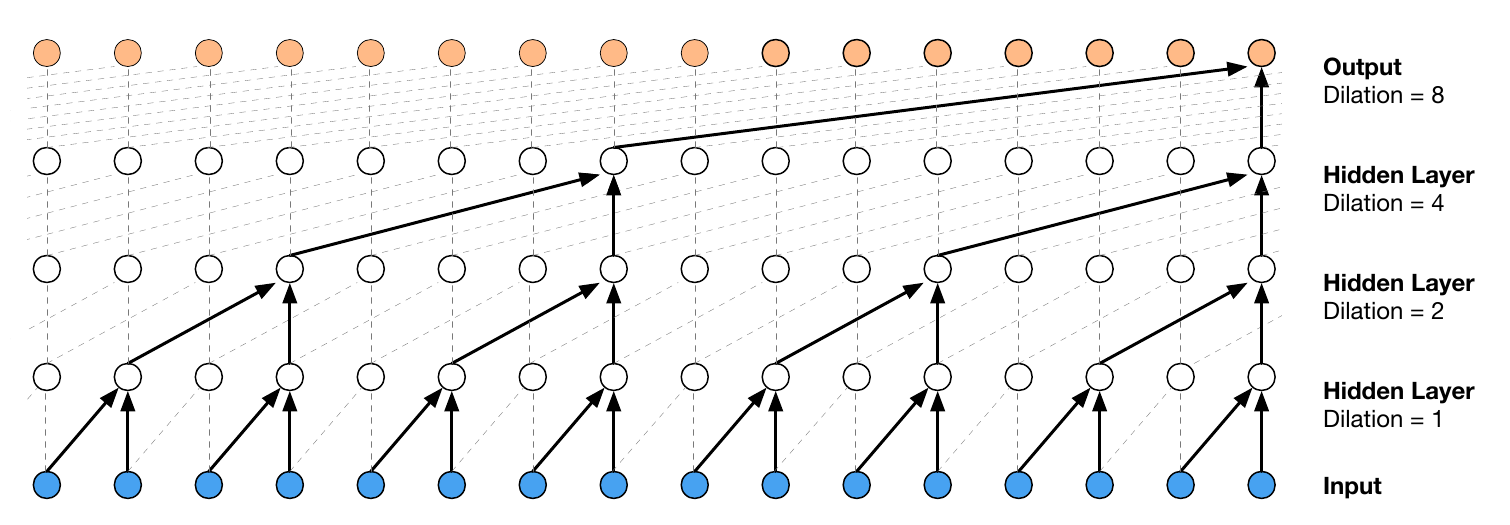
\includegraphics[scale=0.3]{img/casual_dilated}
  \caption{Дырявая свёртка}
  \label{fig:casual_dilated}
\end{figure}

% 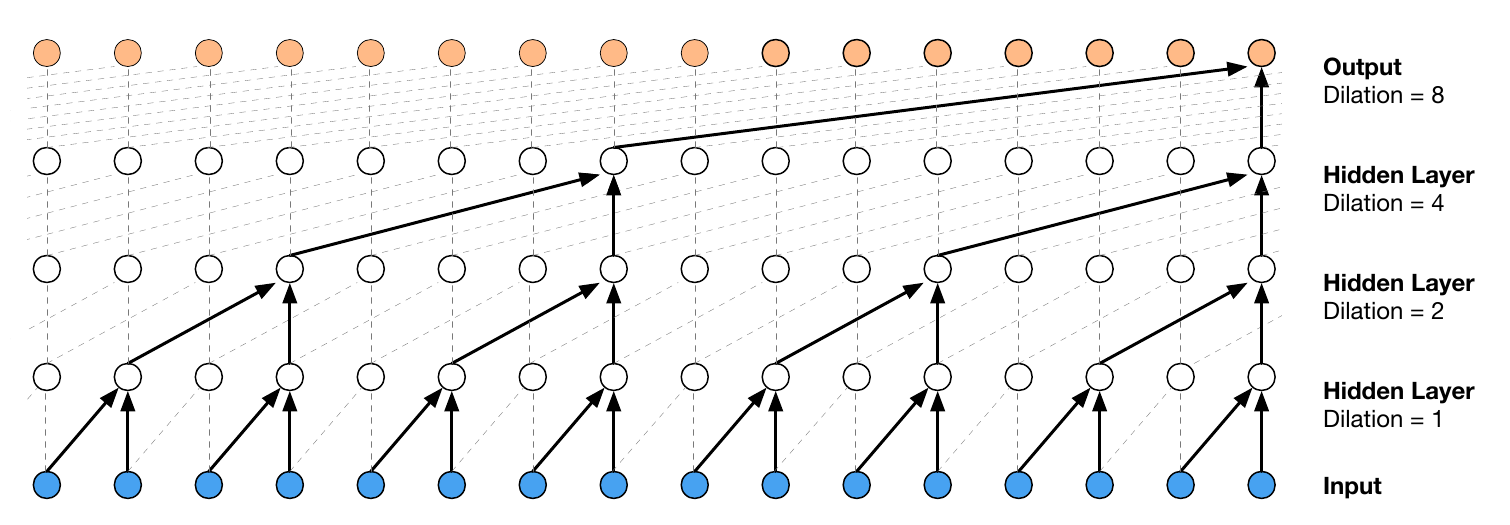
\includegraphics[scale=0.3]{img/casual_dilated}
Главный ингредиент WaveNet - casual свёртки. Используя casual свёртки, мы гарантируем, что модель не может нарушить первоначальный порядок данных: предсказание $p(x_{t+1} = x_1, \dots, x_{t})$ выдаваемое моделью в момент времени $t$ не может зависеть ни от каких моментов в будущем $x_{t+1}, x{t+2}, \dots, x_{T}$. Вы это можете наблюдать на рисунке 1.

Во время обучения условные вероятности во все моменты времени могут вычисляться параллельно, потому что ... Во время генерации предсказания последовательны: каждая предсказанная точка подаётся обратно на вход нейросети, чтобы предсказать следующую.

Поскольку модели с casual свёртками не имеют рекуррентных соединений, они обычно обучаются быстрее нежели рекуррентные архитектуры, особенно когда применяеются к длинным последовательностям. Одна из проблем casual свёрток в том, что они требуют большое количество слоёв либо большие фильтры, чтобы увеличить ширину захватываемого окна. Например, на рисунке 1 ширина захватываемого окна равна 5 (=\#слоёв + длина фильтра - 1). Для решения этой проблемы и появились свёртки с дырками, позволяющие на порядки увеличить ширину окна, не накладывая слишком больших вычислительных затрат. 

Дырявые свёртки это свёртки, в которых фильр применяется по диапазону больше своей длины, пропуская входные значения с некотрым шагом. Что эквиваленто свёртке с больим фильтром, "продырявленным" нулями, но значительно эффективнее вычислительно. Такая эффективность дырявых свёрток позовляет нейросети оперировать c более крупным данными, нежели позволили бы обычные свёртки. В частном случае дыряве свёртки с пропуском 1 эквиваленты обычным свёрткам. На рисунке 2 изображены дырявые свёртки с промежутками 1, 2, 4 и 8. 

\begin{figure}[h!]
  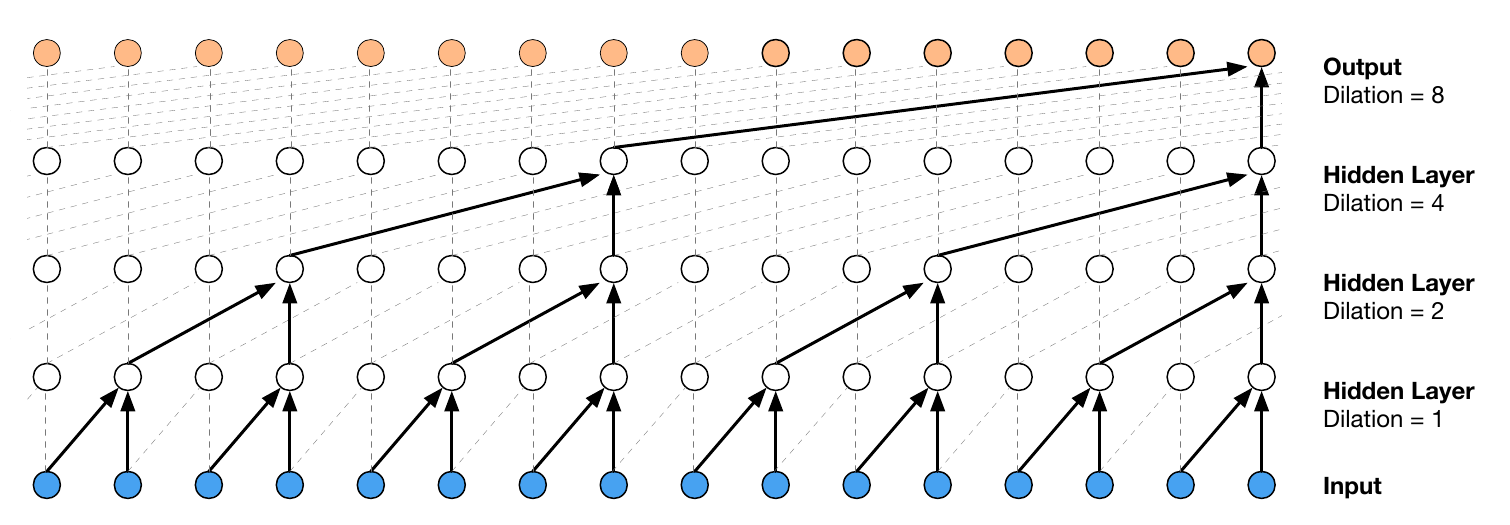
\includegraphics[scale=0.3]{img/casual_dilated}
  \caption{Дырявая свёртка}
  \label{fig:casual_dilated}
\end{figure}

Пачки дырявых свёрток позовляют достичь очень большого ... окна с помощью небольшого количества слоёв, при этом сохраняя качество входныез данных вдоль всей сети. В оригинальном WaveNet промежути увеливчиваются в два раза для каждого слоя пока не достигнут какого-то фиксированного значия, и затем всё повторояется. Например:
$$1,2,4,\dots, 512, 1,2,4,\dots, 512, 1,2,4,\dots, 512.$$ 

Попробуем объяснить интуицию за такой конфигурацией. Во-первых, экспоненциальное увеличение промежутков приводит к экспоненциальному по глубине росту окна. \cite{arxiv:yu-fisher} Например, каждый $1,2,4, \dots 512$ блок имеет окно размера $1024$ его можно воспринимать в качестве более эффектиной и имеющей большую описательную силу(не линейный) альтернативы свёртки $1 \times 1024$. Во-вторых, дальнейшее объединение таких слоёв в пачки увеличивает объём модели и ширину окна.

\newpage
\subsection{Gated activation unit}
Gated activation unit выглядит так:
$$z = \tanh(W_{f,k} * x \  \astrosun \  \sigma(W_{g,k} * x))$$
где $*$ обозначает операцию свёртки, $\astrosun$ обозначает поэлементное умножение, $\sigma(\cdot)$ сигмоида, $k$ номер слоя, $f$ и $g$ обозначают filter и gate соответсвенно, и $W$ обучаемый свёрточный filter. Авторы WaveNet утверждают, что такая функция активации работает занчительно лучше для генерации аудиосигналов чем стандартная rectified linear activation function.

\subsection{Residual и skip соединения}

\begin{figure}[h!]
  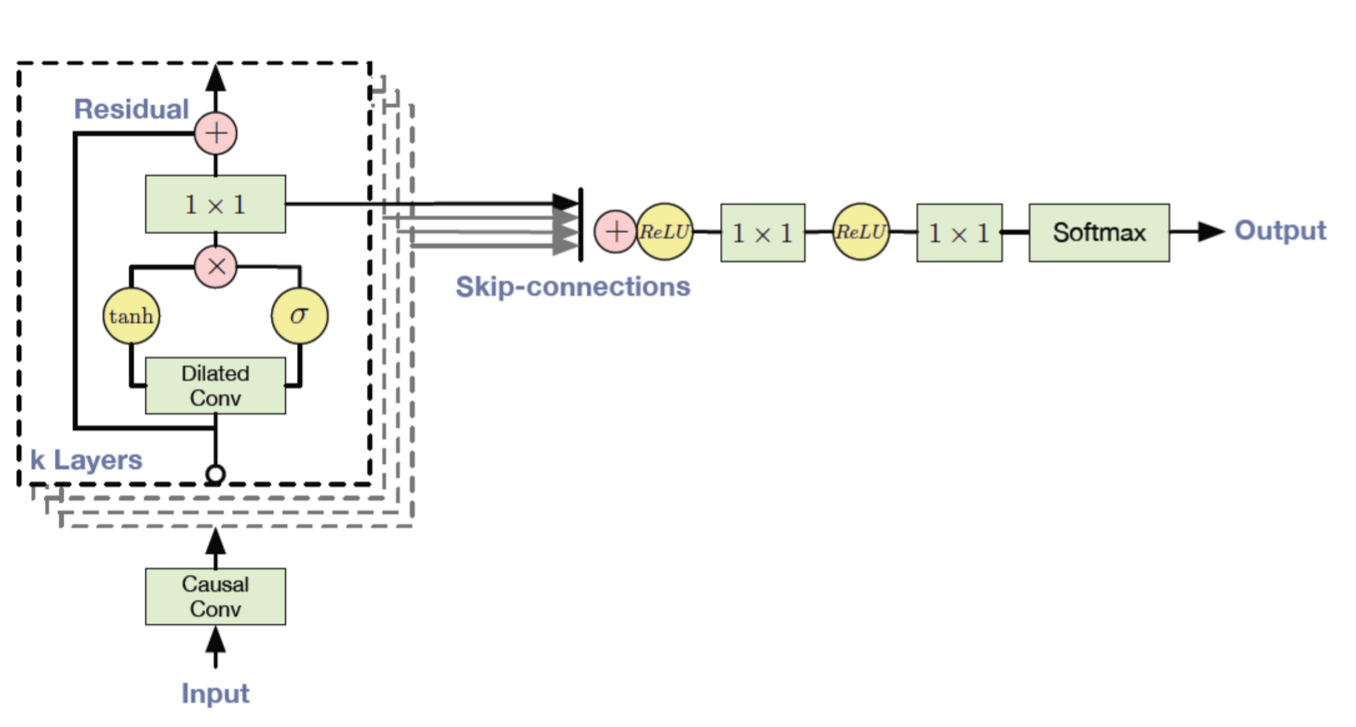
\includegraphics[scale=0.4]{img/wavenet}
  \caption{Архитектура WaveNet}
  \label{fig:wavenet_arch}
\end{figure}

% 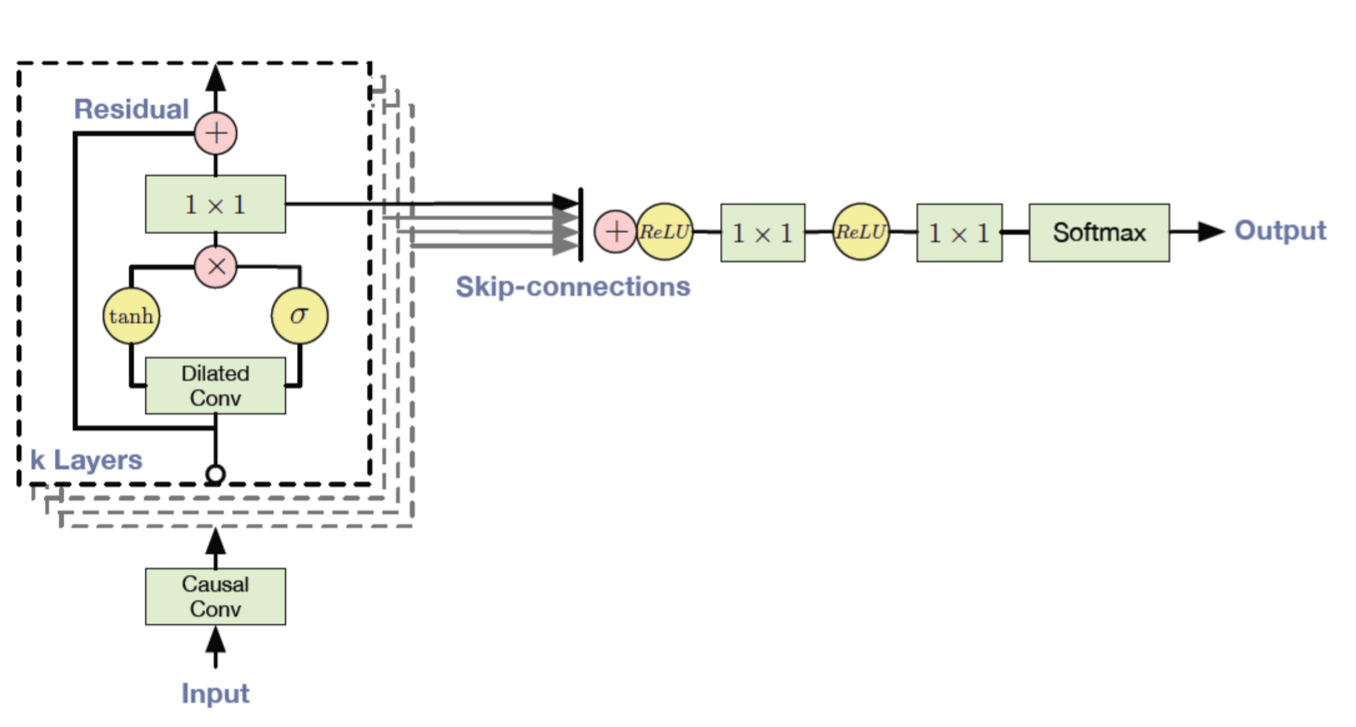
\includegraphics[scale=0.4]{img/wavenet}
В архитектуре используются residual и параметрически skip соединения чтобы ускорить сходимость и позволить обучение более глубокий моделей. На рисунке показан residual блок модели, который повторояется много раз в архитектуре. 


\end{document}

